\documentclass[12pt,a4paper,UTF8]{book}
\usepackage{geometry}   %页边距调整
\geometry{left=2.0cm,right=2.0cm,top=2.5cm,bottom=2.5cm}
\usepackage[hyperref, UTF8]{ctex}   %中文输入,及生成PDF时自动生成书签
\hypersetup{colorlinks=true,linkcolor=black}   %取消目录的默认红框显示
\usepackage{makeidx}
\usepackage{pgf}   %创建PostScript和pdf格式的图形
\usepackage{tikz}   %配合pgf宏包创建复杂图表,例如函数图像
\usetikzlibrary{math}   %tikz宏包中的库,用于在画图时自己创建变量
\usepackage{extpfeil}   %extpfeil扩展添加了更多用于生成可扩展箭头的宏,例如\xlongequal等
\usepackage{txfonts}   %数学字符库
\usepackage{amsmath}   %更好的数学排版环境,里面提供了更多函数,例如\text{}、\operatorname{}等
\usepackage{latexsym}   %使用不同的符号字体宏包
\usepackage{longtable}   %可换页表格
\usepackage{graphicx}   %可导入和调整外部图片
\usepackage{enumerate}   %自定义编号标签

\begin{document}
\frontmatter
\title{概率论与数理统计笔记}
\author{衔瑜\thanks{Email: fish233yeah@163.com}}
\date{\today}
\maketitle
\tableofcontents



\mainmatter
\setlength{\parindent}{0pt}
\chapter{知识点总结}

\section{随机事件及其概率}
\subsection{基本知识}
\begin{enumerate}
\item \textbf{样本空间与样本点}:对于随机事件$E$,它的所有可能结果组成的集合即为$E$的样本空间,通常记为$S$;而样本空间中的元素(即$E$的每个结果)则称为样本点
\item \textbf{摩根率(对偶率)}:$\overline{A+B}=\overline{A}\,\overline{B}$,$\overline{AB}=\overline{A}+\overline{B}$
\item \textbf{排列组合公式}:$A_n^m=\frac{n!}{\left(n-m\right)!}$,$C_n^m=\frac{A_n^m}{m!}$。此外我们有:$C_n^m=C_n^{n-m}$和$C_n^m=C_{n-1}^m+C_{n-1}^{m-1}$
\item \textbf{条件概率}:称$P\left(B|A\right)=\frac{P\left(AB\right)}{P\left(A\right)}$为事件$B$在事件$A$发生的条件下发生的概率。而对于多个事件$B_1,B_2,\cdots$,若它们为两两互不相容的事件,则我们有$P\left(\bigcup\limits_{i=1}^{\infty}B_i|A\right)=\sum\limits_{i=1}^{\infty}P\left(B_i|A\right)$
\item \textbf{全概率公式}:设$E$的样本空间为$S$,$A$为$E$的事件,$B_1,B_2,\cdots,B_n$为$S$的一个划分,且$P\left(B_i\right)>0$,则有:
\[P\left(A\right)=P\left(A|B_1\right)P\left(B_1\right)+P\left(A|B_2\right)P\left(B_2\right)+\cdots+P\left(A|B_n\right)P\left(B_n\right)\]
\item \textbf{贝叶斯公式}:设$E$的样本空间为$S$,$A$为$E$的事件,$B_1,B_2,\cdots,B_n$为$S$的一个划分,且$P\left(A\right)>0$,$P\left(B_i\right)>0$,则有:
\[P\left(B_i|A\right)=\frac{P\left(A|B_i\right)P\left(B_i\right)}{\sum\limits_{j=1}^nP\left(A|B_j\right)P\left(B_j\right)}\]
\item \textbf{事件独立定义}:设$A_1,A_2,\cdots,A_n$为$n$个事件,若对于其中任意$2$个、任意$3$个、$\cdots$、任意$n$个事件的积事件的概率都等于各事件概率之积,则称事件$A_1,A_2,\cdots,A_n$相互独立
\item 若非负实数$k_1,k_2,\cdots,k_n$满足$k_1+k_2+\cdots+k_n=1$,则分布函数$F_1\left(x\right),F_2\left(x\right),\cdots,F_n\left(x\right)$的线性组合$F\left(x\right)=k_1F_1\left(x\right)+k_2F_2\left(x\right)+\cdots+k_nF_n\left(x\right)$仍为某一随机变量的分布函数
\end{enumerate}


\section{计算事件的概率}
\subsection{部分公式}
\begin{enumerate}[]
\item $P\left(A-B\right)=P\left(A\right)-P\left(AB\right)$\\
$P\left(A+B\right)=P\left(A\right)+P\left(B\right)-P\left(AB\right)$\\
$P\left(A+B+C\right)=P\left(A\right)+P\left(B\right)+P\left(C\right)-P\left(AB\right)-P\left(AC\right)-P\left(BC\right)+P\left(ABC\right)$\\
$P\left(A_1+A_2+\cdots+A_n\right)=\sum\limits_{i=1}^nP\left(A_i\right)-\sum\limits_{1\leq i<j\leq n}P\left(A_iA_j\right)+\cdots+\left(-1\right)^{n-1}P\left(A_1A_2\cdots A_n\right)$\\
$P\left(AB\right)=P\left(A\right)P\left(B|A\right)=P\left(B\right)P\left(A|B\right)$\\
$P\left(A_1A_2\cdots A_n\right)=P\left(A_1\right)P\left(A_2|A_1\right)P\left(A_3|A_1A_2\right)\cdots P\left(A_n|A_1A_2\cdots A_{n-1}\right)$\\
\end{enumerate}


\section{随机变量及其分布}
\subsection{几种离散型随机变量分布律}
\begin{enumerate}
\item \textbf{两点分布}:又称为伯努利分布、$(0-1)$分布,随机变量$X$只可能取$0$和$1$两个值,分布律为:
\[P\left\{X=k\right\}=p^k\left(1-p\right)^{1-k},\quad k=0,1\]
\item \textbf{二项分布}:设试验$E$只有两个可能的结果$A$和$\overline{A}$,$P\left(A\right)=p$,则称$E$为伯努利试验,我们将试验$E$独立重复$n$次的话则称其为$n$重伯努利试验。现在假设我们用$X$表示$n$重伯努利试验中事件$A$发生的次数,则其符合二项分布,记为$X\sim b\left(n,p\right)$或$X\sim B\left(n,p\right)$,分布律为:
\[P\left\{X=k\right\}=C_{n}^{k}p^k\left(1-p\right)^{n-k},\quad k=0,1,2,\cdots,n\]
\item \textbf{泊松分布}:设随机变量$X$所有可能取的值为$0,1,2,\cdots$,分布率为:
\[P\left\{X=k\right\}=\frac{\lambda^ke^{-\lambda}}{k!},\quad k=0,1,2,\cdots\]
其中$\lambda>0$,此时我们称随机变量$X$服从参数为$\lambda$的泊松分布,记为$X\sim \pi\left(\lambda\right)$或$X\sim P\left(\lambda\right)$。此外,若我们记$np_n=\lambda$,我们还有泊松定理:
\[\lim\limits_{n\to\infty}C_{n}^{k}p_n^k\left(1-p_n\right)^{n-k}=\frac{\lambda^ke^{-\lambda}}{k!}\]
\item \textbf{几何分布}:设在伯努利试验中事件$A$发生的概率为$p$,若记事件$A$首次发生时的经历的试验总次数为$X$,则我们称随机变量$X$服从参数为$p$的几何分布,分布律为:
\[P\left\{X=k\right\}=pq^{k-1},\quad k=1,2,\cdots\]
\item \textbf{超几何分布}:设在$N$个物品中有$N_1$个次品,从中任取$n(1\leq n\leq N_1)$个,设$X$为这$n$个物品中的次品的数量,则随机变量$X$服从超几何分布,分布律为:
\[P\left\{X=k\right\}=\frac{C_{N_1}^kC_{N-N_1}^{n-k}}{C_N^n}\]
\end{enumerate}

\subsection{几种连续型随机变量分布律}
\begin{enumerate}
\item \textbf{均匀分布}:记为$X\sim U\left(a,b\right)$
\[f\left(x\right)=\left\{\begin{matrix}
\dfrac{1}{b-a}\ ,&a<x<b\\
0\ ,&else
\end{matrix}\right.\]
\[F\left(x\right)=\left\{\begin{matrix}
0\ ,&x<a\\
\dfrac{x-a}{b-a}\ ,&a\leq x<b\\
1\ ,&x\geq b
\end{matrix}\right.\]
\item \textbf{指数分布}:记服从参数$\lambda>0$的指数分布为$X\sim E\left(\lambda\right)$或$X\sim Exp\left(\lambda\right)$
\[f\left(x\right)=\left\{\begin{matrix}
\lambda e^{-\lambda x}\ ,&x\geq0\\
0\ ,&x<0
\end{matrix}\right.\]
\[F\left(x\right)=\left\{\begin{matrix}
1-e^{-\lambda x}\ ,&x\geq0\\
0\ ,&x<0
\end{matrix}\right.\]
指数分布具有无记忆性,即:
\[P\left(X>s+t|X>s\right)=P\left(X>t\right)\]
\item \textbf{正态分布}:又叫做高斯分布,记服从参数$\mu,\sigma\left(\sigma>0\right)$的正态分布为$X\sim N\left(\mu,\sigma^2\right)$
\[f\left(x\right)=\frac{1}{\sqrt{2\pi}\sigma}e^{-\frac{\left(x-\mu\right)^2}{2\sigma^2}},\quad-\infty<x<\infty\]
\[F\left(x\right)=\frac{1}{\sqrt{2\pi}\sigma}\int_{-\infty}^{x}e^{-\frac{\left(t-\mu\right)^2}{2\sigma^2}}dt,\quad-\infty<x<\infty\]
当$\mu=0$,$\sigma=1$时称随机变量$X$服从标准正态分布,其概率密度函数和分布函数为
\[f\left(x\right)=\frac{1}{\sqrt{2\pi}}e^{-\frac{x^2}{2}},\quad-\infty<x<\infty\]
\[F\left(x\right)=\frac{1}{\sqrt{2\pi}}\int_{-\infty}^{x}e^{-\frac{t^2}{2}}dt,\quad-\infty<x<\infty\]
正态分布有如下几个性质:
\begin{enumerate}
\item 正态分布$N\left(\mu,\sigma^2\right)$的数学期望为$\mu$,方差为$\sigma^2$
\item 若$X\sim N\left(\mu,\sigma^2\right)$,则$Y=\frac{X-\mu}{\sigma}\sim N\left(0,1\right)$
\item 若$X\sim N\left(\mu,\sigma^2\right)$,则$Y=aX+b\sim N\left(a\mu+b,\left(a\sigma\right)^2\right),\,a\neq0$
\item 若$X_i\sim N\left(\mu_i,\sigma_i^2\right),\,\left(i=1,2,\cdots,n\right)$,且$X_1,X_2,\cdots,X_n$相互独立,则其线性组合$Y=a_1X_1\pm a_2X_2\pm\cdots\pm a_nX_n$仍服从正态分布,且有
\[Y\sim N\left(a_1\mu_1\pm a_2\mu_2\pm\cdots\pm a_n\mu_n,a_1^2\sigma_1^2+a_2^2\sigma_2^2+\cdots+a_n^2\sigma_n^2\right)\]
\end{enumerate}
\end{enumerate}

\subsection{完整概率分布表}
\begin{scriptsize}
\begin{center}
\begin{longtable}{|c|c|c|c|c|}\hline
分布&参数&分布律或概率密度函数&期望&方差\\
\hline
(0-1)分布&
$0<p<1$&
$P\left\{X=k\right\}=p^k\left(1-p\right)^{1-k},\ k=0,1$&
$p$&
$p\left(1-p\right)$\\
\hline
二项分布&
$\begin{matrix}n\geq1\\0<p<1\end{matrix}$&
$\begin{matrix}P\left\{X=k\right\}=C_{n}^{k}p^k\left(1-p\right)^{n-k}\\k=0,1,2,\cdots,n\end{matrix}$&
$np$&
$np\left(1-p\right)$\\
\hline
$\begin{matrix}\text{负二项分布}\\\text{(帕斯卡分布)}\end{matrix}$&
$\begin{matrix}r\geq1\\0<p<1\end{matrix}$&
$\begin{matrix}P\left\{X=k\right\}=C_{k-1}^{r-1}p^r\left(1-p\right)^{k-r}\\k=r,r+1,\cdots\end{matrix}$&
$\dfrac{r}{p}$&
$\dfrac{r\left(1-p\right)}{p^2}$\\
\hline
几何分布&
$0<p<1$&
$\begin{matrix}P\left\{X=k\right\}=p\left(1-p\right)^{k-1}\\k=1,2,\cdots\end{matrix}$&
$\dfrac{1}{p}$&
$\dfrac{1-p}{p^2}$\\
\hline
超几何分布&
$\begin{matrix}N,\ M,\ n\\\left(M\leq N\right)\\\left(n\leq N\right)\end{matrix}$&
$\begin{matrix}P\left\{X=k\right\}=\dfrac{C_{M}^{k}\cdot C_{N-M}^{n-k}}{C_{N}^{k}}\\\max\left\{0,n-N+M\right\}\leq k\leq\min\left\{n,M\right\}\end{matrix}$&
$\dfrac{nM}{N}$&
$\dfrac{nM}{N}\left(1-\dfrac{M}{N}\right)\left(\dfrac{N-n}{N-1}\right)$\\
\hline
泊松分布&
$\lambda>0$&
$\begin{matrix}P\left\{X=k\right\}=\dfrac{\lambda^ke^{-\lambda}}{k!}\\k=0,1,2,\cdots\end{matrix}$&
$\lambda$&
$\lambda$\\
\hline
均匀分布&
$a<b$&
$f\left(x\right)=\left\{\begin{matrix}\dfrac{1}{b-a}\ ,&a<x<b\\0\ ,&else\end{matrix}\right.$&
$\dfrac{a+b}{2}$&
$\dfrac{\left(b-a\right)^2}{12}$\\
\hline
正态分布&
$\begin{matrix}\mu\\\sigma>0\end{matrix}$&
$f\left(x\right)=\dfrac{1}{\sqrt{2\pi}\sigma}e^{-\frac{\left(x-\mu\right)^2}{2\sigma^2}}$&
$\mu$&
$\sigma^2$\\
\hline
$\Gamma$分布&
$\begin{matrix}\alpha>0\\\beta>0\end{matrix}$&
$f\left(x\right)=\left\{\begin{matrix}\dfrac{1}{\beta^{\alpha}\Gamma\left(\alpha\right)}x^{\alpha-1}e^{-\frac{x}{\beta}}\ ,&x>0\\0\ ,&else\end{matrix}\right.$&
$\alpha\beta$&
$\alpha\beta^2$\\
\hline
$\begin{matrix}\text{指数分布}\\\text{(负指数分布)}\end{matrix}$&
$\lambda>0$&
$f\left(x\right)=\left\{\begin{matrix}\lambda e^{-\lambda x}\ ,&x\geq0\\0\ ,&x<0\end{matrix}\right.$&
$\dfrac{1}{\lambda}$&
$\dfrac{1}{\lambda^2}$\\
\hline
$\chi^2$分布&
$n\geq1$&
$f\left(x\right)=\left\{\begin{matrix}\dfrac{1}{2^{\frac{n}{2}}\Gamma\left(\frac{n}{2}\right)}x^{\frac{n}{2}-1}e^{-\frac{x}{2}}\ ,&x>0\\0\ ,&else\end{matrix}\right.$&
$n$&
$2n$\\
\hline
韦布尔分布&
$\begin{matrix}\eta>0\\\beta>0\end{matrix}$&
$f\left(x\right)=\left\{\begin{matrix}\dfrac{\beta}{\eta}\left(\dfrac{x}{\eta}\right)^{\beta-1}e^{-\left(\frac{x}{\eta}\right)^{\beta}}\ ,&x>0\\0\ ,&else\end{matrix}\right.$&
$\eta\Gamma\left(\dfrac{1}{\beta}+1\right)$&
$\eta^2\left\{\Gamma\left(\dfrac{2}{\beta}+1\right)-\left[\Gamma\left(\dfrac{1}{\beta}+1\right)\right]^2\right\}$\\
\hline
瑞利分布&
$\sigma>0$&
$f\left(x\right)=\left\{\begin{matrix}\dfrac{x}{\sigma^2}e^{-\frac{x^2}{2\sigma^2}}\ ,&x>0\\0\ ,&else\end{matrix}\right.$&
$\sqrt{\dfrac{\pi}{2}}\sigma$&
$\dfrac{4-\pi}{2}\sigma^2$\\
\hline
$\beta$分布&
$\begin{matrix}\alpha>0\\\beta>0\end{matrix}$&
$f\left(x\right)=\left\{\begin{matrix}\dfrac{\Gamma\left(\alpha+\beta\right)}{\Gamma\left(\alpha\right)\Gamma\left(\beta\right)}x^{\alpha-1}\left(1-x\right)^{\beta-1}\ ,&0<x<1\\0\ ,&else\end{matrix}\right.$&
$\dfrac{\alpha}{\alpha+\beta}$&
$\dfrac{\alpha\beta}{\left(\alpha+\beta\right)^2\left(\alpha+\beta+1\right)}$\\
\hline
对数正态分布&
$\begin{matrix}\mu\\\sigma>0\end{matrix}$&
$f\left(x\right)=\left\{\begin{matrix}\dfrac{1}{\sqrt{2\pi}\sigma x}e^{-\frac{\left(\ln x-\mu\right)^2}{2\sigma^2}}\ ,&x>0\\0\ ,&else\end{matrix}\right.$&
$e^{\mu+\frac{\sigma^2}{2}}$&
$e^{2\mu+\sigma^2}\left(e^{\sigma^2}-1\right)$\\
\hline
柯西分布&
$\begin{matrix}a\\\lambda>0\end{matrix}$&
$f\left(x\right)=\dfrac{1}{\pi}\cdot\dfrac{\lambda}{\lambda^2+\left(x-a\right)^2}$&
不存在&
不存在\\
\hline
$t$分布&
$n\geq1$&
$f\left(x\right)=\dfrac{\Gamma\left(\dfrac{n+1}{2}\right)}{\sqrt{n\pi}\cdot\Gamma\left(\dfrac{n}{2}\right)}\left(1+\dfrac{x^2}{n}\right)^{-\frac{n+1}{2}}$&
$0,n>1$&
$\dfrac{n}{n-2},n>2$\\
\hline
$F$分布&
$n_1,n_2$&
$f\left(x\right)=\left\{\begin{matrix}\dfrac{\Gamma\left(\dfrac{n_1+n_2}{2}\right)\cdot\left(\dfrac{n_1}{n_2}\right)^{\frac{n_1}{2}}\cdot x^{\frac{n_1}{2}-1}}{\Gamma\left(\dfrac{n_1}{2}\right)\cdot\Gamma\left(\dfrac{n_2}{2}\right)\cdot\left(1+\dfrac{n_1}{n_2}x\right)^{\frac{n_1+n_2}{2}}}\ ,&x>0\\0\ ,&else\end{matrix}\right.$&
$\begin{matrix}\dfrac{n_2}{n_2-2}\\n_2>2\end{matrix}$&
$\begin{matrix}\dfrac{2n_2^2\left(n_1+n_2-2\right)}{n_1\left(n_2-2\right)^2\left(n_2-4\right)}\\n_2>4\end{matrix}$\\
\hline
\caption{概率分布表}
\label{tab:Margin_settings}
\end{longtable}
\end{center}
\end{scriptsize}


\section{多维随机变量及其分布}
\subsection{边缘分布}
\begin{enumerate}
\item \textbf{离散型随机变量边缘分布}:
\[p_{i\cdot}=P\left\{X=x_i\right\}=\sum\limits_{j=1}^{\infty}p_{ij}\]
\[p_{\cdot j}=P\left\{Y=y_j\right\}=\sum\limits_{i=1}^{\infty}p_{ij}\]
\item \textbf{连续型随机变量边缘分布}:
\[f_X\left(x\right)=\int_{-\infty}^{\infty}f\left(x,y\right)dy\]
\[f_Y\left(y\right)=\int_{-\infty}^{\infty}f\left(x,y\right)dx\]
\end{enumerate}

\subsection{条件分布}
\begin{enumerate}
\item \textbf{离散型随机变量条件分布}:
\[P\left\{X=x_i|Y=y_j\right\}=\frac{P\left\{X=x_i,Y=y_j\right\}}{P\left\{Y=y_j\right\}}=\frac{p_{ij}}{p_{\cdot j}}\]
\[P\left\{Y=y_j|X=x_i\right\}=\frac{P\left\{X=x_i,Y=y_j\right\}}{P\left\{X=x_i\right\}}=\frac{p_{ij}}{p_{i\cdot}}\]
\item \textbf{连续型随机变量条件分布}:
\[f_{X|Y}\left(x|y\right)=\frac{f\left(x,y\right)}{f_Y\left(y\right)}\]
\[f_{Y|X}\left(y|x\right)=\frac{f\left(x,y\right)}{f_X\left(x\right)}\]
\end{enumerate}

\subsection{二维随机变量独立性}
\begin{enumerate}
\item 设$F\left(x,y\right)$及$F_X\left(x\right)$,$F_Y\left(y\right)$分别是二维随机变量$\left(X,Y\right)$的分布函数及边缘分布函数,则随机变量$X$和$Y$相互独立的两个相互等价的条件为:
\begin{enumerate}
\item $F\left(x,y\right)=F_X\left(x\right)F_Y\left(y\right)$在平面上恒成立
\item $f\left(x,y\right)=f_X\left(x\right)f_Y\left(y\right)$在平面上几乎处处成立
\end{enumerate}
当随机变量$X$和$Y$相互独立时,显然我们有:
\[f_{X|Y}\left(x|y\right)=\frac{f\left(x,y\right)}{f_Y\left(y\right)}=\frac{f_X\left(x\right)f_Y\left(y\right)}{f_Y\left(y\right)}=f_X\left(x\right)\]
\[f_{Y|X}\left(y|x\right)=\frac{f\left(x,y\right)}{f_X\left(x\right)}=\frac{f_X\left(x\right)f_Y\left(y\right)}{f_X\left(x\right)}=f_Y\left(y\right)\]
即二维随机变量$X,Y$相互独立的充要条件为$X,Y$的所有条件分布都与其边缘分布相同
\item 设多维随机变量$\left(X_1,X_2,\cdots,X_m\right)$和$\left(Y_1,Y_2,\cdots,Y_n\right)$相互独立,则$X_i$和$Y_j$相互独立。又若$h$,$g$是连续函数,则$h\left(X_1,X_2,\cdots,X_m\right)$和$g\left(Y_1,Y_2,\cdots,Y_n\right)$相互独立
\item 独立一定不相关,不相关不一定独立
\end{enumerate}

\subsection{二维随机变量函数$Z=g\left(X,Y\right)$的分布}
\begin{enumerate}
\item 离散型随机变量函数概率分布计算:
\[P\left(Z=z_k\right)=P\left(g\left(X,Y\right)=z_k\right)=\sum\limits_{g\left(x_i,y_j\right)=z_k}p_{ij}\]
\item 连续型随机变量函数概率分布计算:
\[P\left(Z=z\right)=P\left(g\left(X,Y\right)\leq z\right)=P\left(\left(X,Y\right)\in G\right)=\iint\limits_{G}f\left(x,y\right)dxdy\]
其中$G=\left\{\left(x,y\right)|g\left(x,y\right)\leq z\right\}$
\end{enumerate}

\subsection{二维均匀分布及二维正态分布的性质}
\begin{enumerate}
\item \textbf{二维均匀分布}
\begin{enumerate}
\item 定义:\\
设$G$为平面上的有界区域,面积为$S\left(G\right)$,若二维随机变量$\left(X,Y\right)$在$G$上服从均匀分布,则
\[f\left(x,y\right)=\left\{\begin{matrix}
\dfrac{1}{S\left(G\right)}\ ,&\left(x,y\right)\in G\\
0\ ,&else
\end{matrix}\right.\]
记为$\left(X,Y\right)\sim U\left(G\right)$
\item 性质:
\begin{enumerate}
\item 设矩形区域为$G=\left\{\left(x,y\right)|a\leq x\leq b,c\leq y\leq d\right\}$,则二维随机变量$\left(X,Y\right)$在矩形区域$G$上服从均匀分布的充分必要条件为$X,Y$分别在$\left(a,b\right),\left(c,d\right)$上分别服从均匀分布
\end{enumerate}
\end{enumerate}
\item \textbf{二维正态分布}
\begin{enumerate}
\item 定义:\\
二维随机变量$\left(X,Y\right)$在平面上服从二维正态分布,则
\[f\left(x,y\right)=\frac{1}{2\pi\sigma_1\sigma_2\sqrt{1-\rho^2}}e^{-\frac{1}{2\left(1-\rho^2\right)}\left[\frac{\left(x-\mu_1\right)^2}{\sigma_1^2}-2\rho\frac{\left(x-\mu_1\right)\left(y-\mu_2\right)}{\sigma_1\sigma_2}+\frac{\left(y-\mu_2\right)^2}{\sigma_2^2}\right]}\]
记为$\left(X,Y\right)\sim N\left(\mu_1,\mu_2,\sigma_1^2,\sigma_2^2,\rho\right)$
\item 性质:
\begin{enumerate}
\item 对于二维正态随机变量$\left(X,Y\right)$,$X$和$Y$相互独立的充分必要条件为$\rho=0$
\item 二维正态随机变量$\left(X,Y\right)\sim N\left(\mu_1,\mu_2,\sigma_1^2,\sigma_2^2,\rho\right)$的边缘密度函数$f_X\left(x\right)$与$f_Y\left(y\right)$与$\rho$的取值无关,恒为
\[f_X\left(x\right)=\frac{1}{\sqrt{2\pi}\sigma_1}e^{-\frac{\left(x-\mu_1\right)^2}{2\sigma_1^2}}\]
\[f_Y\left(y\right)=\frac{1}{\sqrt{2\pi}\sigma_2}e^{-\frac{\left(y-\mu_2\right)^2}{2\sigma_2^2}}\]
即若$\left(X,Y\right)$服从二维正态分布,则$X$和$Y$都服从一维正态分布
\item 若$X$和$Y$都服从一维正态分布,且$X$和$Y$相互独立,则$\left(X,Y\right)$服从二维正态分布
\item $\left(X,Y\right)$服从二维正态分布的充分必要条件为$X$和$Y$的任意线性组合$l_1X+l_2Y$($l_1,l_2$不全为零)均服从一维正态分布
\item (正态变量线性变换不变性)若$\left(X,Y\right)$服从二维正态分布,记随机变量
\[U=aX+bY,\ V=cX+dY,\ \text{且}\begin{vmatrix}a&b\\c&d\end{vmatrix}\neq0\]
则$\left(U,V\right)$也服从二维正态分布
\end{enumerate}
\end{enumerate}
\end{enumerate}


\section{随机变量的数字特征}
\subsection{期望定义}
\begin{enumerate}
\item 定义:
\begin{enumerate}
\item 对于离散型随机变量$X$,设分布律为$P\left(X=x_k\right)=p_k,\ k=1,2,\cdots$,若级数$\sum\limits_{k=1}^{\infty}x_kp_k$绝对收敛,则$X$的期望定义为
\[E\left(X\right)=\sum\limits_{k=1}^{\infty}x_kp_k\]
\item 对于连续型随机变量$X$,设概率密度函数为$f\left(x\right)$,若积分$\int_{-\infty}^{+\infty}xf\left(x\right)dx$绝对收敛,则$X$的期望定义为
\[E\left(X\right)=\int_{-\infty}^{+\infty}xf\left(x\right)dx\]
\end{enumerate}
\item 一维随机变量函数期望:\\
设函数$g\left(x\right)$连续,则随机变量$Y=g\left(X\right)$的期望如下
\begin{enumerate}
\item 对于离散型随机变量$X$,设分布律为$P\left(X=x_k\right)=p_k,\ k=1,2,\cdots$,若级数$\sum\limits_{k=1}^{\infty}g\left(x_k\right)p_k$绝对收敛,则有
\[E\left(Y\right)=E\left[g\left(X\right)\right]=\sum\limits_{k=1}^{\infty}g\left(x_k\right)p_k\]
\item 对于连续型随机变量$X$,设概率密度函数为$f\left(x\right)$,若积分$\int_{-\infty}^{+\infty}g\left(x\right)f\left(x\right)dx$绝对收敛,则有
\[E\left(Y\right)=E\left[g\left(X\right)\right]=\int_{-\infty}^{+\infty}g\left(x\right)f\left(x\right)dx\]
\end{enumerate}
\item 二维随机变量函数期望:\\
设函数$g\left(x,y\right)$连续,则随机变量$Z=g\left(X,Y\right)$的期望如下
\begin{enumerate}
\item 对于二维离散型随机变量$\left(X,Y\right)$,设分布律为$P\left(X=x_i,Y=y_j\right)=p_{ij},\ i,j=1,2,\cdots$,若级数$\sum\limits_{i=1}^{\infty}\sum\limits_{j=1}^{\infty}g\left(x_i,y_j\right)p_{ij}$绝对收敛,则有
\[E\left(Z\right)=E\left[g\left(X,Y\right)\right]=\sum\limits_{i=1}^{\infty}\sum\limits_{j=1}^{\infty}g\left(x_i,y_j\right)p_{ij}\]
特别地,我们有
\[E\left(X\right)=\sum\limits_{i=1}^{\infty}\sum\limits_{j=1}^{\infty}x_ip_{ij}=\sum\limits_{i=1}^{\infty}x_ip_{i\cdot}\]
\[E\left(Y\right)=\sum\limits_{i=1}^{\infty}\sum\limits_{j=1}^{\infty}y_jp_{ij}=\sum\limits_{j=1}^{\infty}y_jp_{\cdot j}\]
\item 对于连续型随机变量$\left(X,Y\right)$,设概率密度函数为$f\left(x,y\right)$,若积分$\int_{-\infty}^{+\infty}\int_{-\infty}^{+\infty}g\left(x,y\right)f\left(x,y\right)dxdy$ 绝对收敛,则有
\[E\left(Z\right)=E\left[g\left(X,Y\right)\right]=\int_{-\infty}^{+\infty}\int_{-\infty}^{+\infty}g\left(x,y\right)f\left(x,y\right)dxdy\]
特别地,我们有
\[E\left(X\right)=\int_{-\infty}^{+\infty}\int_{-\infty}^{+\infty}xf\left(x,y\right)dxdy=\int_{-\infty}^{+\infty}xf_X\left(x\right)dx\]
\[E\left(Y\right)=\int_{-\infty}^{+\infty}\int_{-\infty}^{+\infty}yf\left(x,y\right)dxdy=\int_{-\infty}^{+\infty}yf_Y\left(y\right)dy\]
\end{enumerate}
\end{enumerate}

\subsection{方差定义}
\begin{enumerate}
\item 定义:随机变量$X$的期望存在时若$E\left[X-E\left(X\right)\right]^2$也存在,则有
\[D\left(X\right)=E\left[X-E\left(X\right)\right]^2=E\left(X^2\right)-\left[E\left(X\right)\right]^2\]
而标准差定义为
\[\sigma\left(X\right)=\sqrt{D\left(X\right)}\]
\begin{enumerate}
\item 对于离散型随机变量$X$,设分布律为$P\left(X=x_k\right)=p_k,\ k=1,2,\cdots$,若其期望$E\left(X\right)$存在,$\sum\limits_{k=1}^{\infty}\left[x_k-E\left(X\right)\right]^2p_k$绝对收敛,则$X$的方差定义为
\[D\left(X\right)=\sum\limits_{k=1}^{\infty}\left[x_k-E\left(X\right)\right]^2p_k\]
\item 对于连续型随机变量$X$,设概率密度函数为$f\left(x\right)$,若其期望$E\left(X\right)$存在,\\$\int_{-\infty}^{+\infty}\left[x-E\left(X\right)\right]^2f\left(x\right)dx$绝对收敛,则$X$的方差定义为
\[D\left(X\right)=\int_{-\infty}^{+\infty}\left[x-E\left(X\right)\right]^2f\left(x\right)dx\]
\end{enumerate}
\item 一维随机变量函数方差:\\
设函数$g\left(x\right)$连续,则随机变量$Y=g\left(X\right)$的方差为
\[D\left(Y\right)=D\left[g\left(X\right)\right]=E\left[g\left(X\right)^2\right]-\left\{E\left[g\left(X\right)\right]\right\}^2\]
\begin{enumerate}
\item 对于离散型随机变量$X$,设分布律为$P\left(X=x_k\right)=p_k,\ k=1,2,\cdots$,若其期望$E\left(X\right)$存在,$\sum\limits_{k=1}^{\infty}\left[g\left(x_k\right)-E\left(X\right)\right]^2p_k$绝对收敛,则$X$的方差定义为
\[D\left(X\right)=\sum\limits_{k=1}^{\infty}\left[g\left(x_k\right)-E\left(X\right)\right]^2p_k\]
\item 对于连续型随机变量$X$,设概率密度函数为$f\left(x\right)$,若其期望$E\left(X\right)$存在,\\$\int_{-\infty}^{+\infty}\left[g\left(x\right)-E\left(X\right)\right]^2f\left(x\right)dx$绝对收敛,则$X$的方差定义为
\[D\left(X\right)=\int_{-\infty}^{+\infty}\left[g\left(x\right)-E\left(X\right)\right]^2f\left(x\right)dx\]
\end{enumerate}
\item 二维随机变量函数方差:\\
设函数$g\left(x,y\right)$连续,则随机变量$Z=g\left(X,Y\right)$的方差为
\begin{enumerate}
\item 对于二维离散型随机变量$\left(X,Y\right)$,设分布律为$P\left(X=x_i,Y=y_j\right)=p_{ij},\ i,j=1,2,\cdots$,若级数$\sum\limits_{i=1}^{\infty}\sum\limits_{j=1}^{\infty}\left\{g\left(x_i,y_j\right)-E\left[g\left(X,Y\right)\right]\right\}^2p_{ij}$绝对收敛,则有
\[D\left(Z\right)=D\left[g\left(X,Y\right)\right]=\sum\limits_{i=1}^{\infty}\sum\limits_{j=1}^{\infty}\left\{g\left(x_i,y_j\right)-E\left[g\left(X,Y\right)\right]\right\}^2p_{ij}\]
特别地,我们有
\[D\left(X\right)=\sum\limits_{i=1}^{\infty}\sum\limits_{j=1}^{\infty}\left[x_i-E\left(X\right)\right]^2p_{ij}=\sum\limits_{i=1}^{\infty}\left[x_i-E\left(X\right)\right]^2p_{i\cdot}\]
\[D\left(Y\right)=\sum\limits_{i=1}^{\infty}\sum\limits_{j=1}^{\infty}\left[y_j-E\left(Y\right)\right]^2p_{ij}=\sum\limits_{j=1}^{\infty}\left[y_j-E\left(Y\right)\right]^2p_{\cdot j}\]
\item 对于连续型随机变量$\left(X,Y\right)$,设概率密度函数为$f\left(x,y\right)$,若积分$\int_{-\infty}^{+\infty}\int_{-\infty}^{+\infty}g\left(x,y\right)f\left(x,y\right)dxdy$ 绝对收敛,则有
\[D\left(Z\right)=D\left[g\left(X,Y\right)\right]=\int_{-\infty}^{+\infty}\int_{-\infty}^{+\infty}\left\{g\left(x,y\right)-E\left[g\left(X,Y\right)\right]\right\}^2f\left(x,y\right)dxdy\]
特别地,我们有
\[D\left(X\right)=\int_{-\infty}^{+\infty}\int_{-\infty}^{+\infty}\left[x-E\left(X\right)\right]^2f\left(x,y\right)dxdy=\int_{-\infty}^{+\infty}\left[x-E\left(X\right)\right]^2f_X\left(x\right)dx\]
\[D\left(Y\right)=\int_{-\infty}^{+\infty}\int_{-\infty}^{+\infty}\left[y-E\left(Y\right)\right]^2f\left(x,y\right)dxdy=\int_{-\infty}^{+\infty}\left[y-E\left(Y\right)\right]^2f_Y\left(y\right)dy\]
\end{enumerate}
\end{enumerate}

\subsection{期望与方差的性质}
\begin{enumerate}
\item $E\left(kX\pm c\right)=kE\left(X\right)\pm c,\ D\left(kX\pm c\right)=k^2D\left(X\right)$
\item $E\left(X_1\pm X_2\right)=E\left(X_1\right)\pm E\left(X_2\right),\ D\left(X_1\pm X_2\right)=D\left(X_1\right)+D\left(X_2\right)\pm\operatorname{Cov}\left(X_1,X_2\right)$
\item 若$X$与$Y$不相关,则有
\[E\left(XY\right)=E\left(X\right)E\left(Y\right)\]
\item 若$X$与$Y$相互独立,则有
\[D\left(XY\right)=D\left(X\right)D\left(Y\right)+\left[E\left(X\right)\right]^2D\left(Y\right)+\left[E\left(Y\right)\right]^2D\left(X\right)\]
\item 若$X$与$Y$相互独立,$g\left(x\right)$和$h\left(x\right)$是两个连续函数,则$U=g\left(X\right)$和$V=h\left(Y\right)$也都是随机变量,且$U$和$V$相互独立
\end{enumerate}

\subsection{协方差与相关系数}
\begin{enumerate}
\item 定义:
\begin{enumerate}
\item 协方差$\operatorname{Cov}\left(X,Y\right)$定义为:
\[\operatorname{Cov}\left(X,Y\right)=E\left\{\left[X-E\left(X\right)\right]\left[Y-E\left(Y\right)\right]\right\}=E\left(XY\right)-E\left(X\right)E\left(Y\right)\]
\begin{enumerate}
\item 二维离散型随机变量协方差:
\[\operatorname{Cov}\left(X,Y\right)=\sum\limits_{i=1}^{\infty}\sum\limits_{j=1}^{\infty}\left[x_i-E\left(X\right)\right]\left[y_j-E\left(Y\right)\right]p_{ij}\]
\item 二维连续型随机变量协方差:
\[\operatorname{Cov}\left(X,Y\right)=\int_{-\infty}^{+\infty}\int_{-\infty}^{+\infty}\left[x-E\left(X\right)\right]\left[y-E\left(Y\right)\right]f\left(x,y\right)dxdy\]
\end{enumerate}
\item 相关系数$\rho_{XY}$定义为:
\[\rho_{XY}=\frac{\operatorname{Cov}\left(X,Y\right)}{\sqrt{D\left(X\right)}\sqrt{D\left(Y\right)}}\]
\end{enumerate}
\item 协方差性质:
\begin{enumerate}
\item $\operatorname{Cov}\left(X,Y\right)=\operatorname{Cov}\left(Y,X\right)$
\item $\operatorname{Cov}\left(X,k\right)=0$,$\operatorname{Cov}\left(k,Y\right)=0$
\item $\operatorname{Cov}\left(aX\pm b,cY\pm d\right)=ac\operatorname{Cov}\left(X,Y\right)$
\item $\operatorname{Cov}\left(X_1\pm X_2,Y\right)=\operatorname{Cov}\left(X_1,Y\right)\pm\operatorname{Cov}\left(X_2,Y\right)$
\end{enumerate}
\item 相关系数性质:
\begin{enumerate}
\item $\left|\rho_{XY}\right|\leq1$
\item $\left|\rho_{XY}\right|=1$的充要条件是,存在常数$a,b$使
\[P\left\{Y=aX+b\right\}=1\]
成立(即相关系数描述的是随机变量的线性相关性,$\rho_{XY}=0$时即表示$X,Y$不相关)
\end{enumerate}
\end{enumerate}

\subsection{矩与协方差矩阵}
\begin{enumerate}
\item \textbf{矩定义}:
\begin{enumerate}
\item $k$阶原点矩:$E\left(X^k\right)$
\item $k$阶中心矩:$E\left\{\left[X-E\left(X\right)\right]^k\right\}$
\item $k+l$阶混合矩:$E\left(X^kY^l\right)$
\item $k+l$阶混合中心矩:$E\left\{\left[X-E\left(X\right)\right]^k\left[Y-E\left(Y\right)\right]^l\right\}$
\end{enumerate}
\item \textbf{协方差矩阵定义}:设$n$维随机变量$\left(X_1,X_2,\cdots,X_n\right)$的协方差
\[c_{ij}=c_{ji}=\operatorname{Cov}\left(X_i,X_j\right)\]
均存在,则称矩阵
\[C=\begin{bmatrix}c_{11}&c_{12}&\cdots&c_{1n}\\c_{21}&c_{22}&\cdots&c_{2n}\\\vdots&\vdots&\ &\vdots\\c_{n1}&c_{n2}&\cdots&c_{nn}\end{bmatrix}\]
为$n$维随机变量$\left(X_1,X_2,\cdots,X_n\right)$的协方差矩阵,显然协方差矩阵为一个对称矩阵
\end{enumerate}

\subsection{其他}
\begin{enumerate}
\item \textbf{切比雪夫不等式}:设随机变量$X$具有数学期望$E\left(X\right)=\mu$,方差$D\left(X\right)=\sigma^2$,则对于任意正数$\varepsilon$,我们有下述不等式成立:
\[P\left\{\left|X-\mu\right|\geq\varepsilon\right\}\leq\frac{\sigma^2}{\varepsilon^2}\]
\end{enumerate}


\section{大数定律与中心极限定理}
\subsection{依概率收敛}
\begin{enumerate}
\item \textbf{定义}:设$X_1,X_2,\cdots$是一个随机变量序列,$a$是一个常数,若对于任意$\varepsilon>0$,有
\[\lim\limits_{n\to\infty}P\left\{\left|X_n-a\right|<\varepsilon\right\}=1\]
则称序列$X_1,X_2,\cdots$依概率收敛于$a$,记为
\[X_n\xrightarrow{\ P\ }a\]
\item \textbf{性质}:设$X_n\xrightarrow{\ P\ }a$,$Y_n\xrightarrow{\ P\ }b$,又函数$g\left(x,y\right)$在点$\left(a,b\right)$处连续,则
\[g\left(X_n,Y_n\right)\xrightarrow{\ P\ }g\left(a,b\right)\]
\end{enumerate}

\subsection{大数定律}
\begin{enumerate}
\item \textbf{大数定律}:设$X_1,X_2,\cdots$为一随机变量序列,若对于任意$\varepsilon>0$,有
\[\lim\limits_{n\to\infty}P\left\{\left|\frac{1}{n}\sum\limits_{k=1}^{n}X_k-E\left(\frac{1}{n}\sum\limits_{k=1}^{n}X_k\right)\right|<\varepsilon\right\}=1\]
则称随机变量序列$X_1,X_2,\cdots$服从大数定律
\item \textbf{切比雪夫大数定律}:设$X_1,X_2,\cdots$是相互独立的随机变量序列,且方差一致有上界,则对于任意$\varepsilon>0$,有
\[\lim\limits_{n\to\infty}P\left\{\left|\frac{1}{n}\sum\limits_{k=1}^{n}X_k-\frac{1}{n}\sum\limits_{k=1}^{n}E\left(X_k\right)\right|<\varepsilon\right\}=1\]
\item \textbf{辛钦大数定律(弱大数定律)}:设$X_1,X_2,\cdots$是相互独立且服从同一分布的随机变量序列,且具有数学期望$E\left(X_k\right)=\mu$,则对于任意$\varepsilon>0$,有
\[\lim\limits_{n\to\infty}P\left\{\left|\frac{1}{n}\sum\limits_{k=1}^{n}X_k-\mu\right|<\varepsilon\right\}=1\]
即$\overline{X}=\frac{1}{n}\sum\limits_{k=1}^{n}X_k$依概率收敛于$\mu$,$\overline{X}\xrightarrow{\ P\ }\mu$
\item \textbf{伯努利大数定律}:设$n_A$是$n$次独立试验中事件$A$发生的次数,$p$是事件$A$在每次试验中发生的概率,则对于任意$\varepsilon>0$,有
\[\lim\limits_{n\to\infty}P\left\{\left|\frac{n_A}{n}-p\right|<\varepsilon\right\}=1\]
即事件$A$发生的频率依概率收敛于事件$A$发生的概率,$\dfrac{n_A}{n}\xrightarrow{\ P\ }p$
\end{enumerate}

\subsection{中心极限定理}
\begin{enumerate}
\item \textbf{李雅普诺夫中心极限定理}:设随机变量序列$X_1,X_2,\cdots$相互独立,且具有期望和方差
\[E\left(X_k\right)=\mu_k,\ D\left(X_k\right)=\sigma_k^2>0\]
则随机变量
\[Z_n=\frac{\sum\limits_{k=1}^{n}X_k-\sum\limits_{k=1}^{n}\mu_k}{\sqrt{\sum\limits_{k=1}^{n}\sigma_k^2}}\]
的分布函数$F_n\left(x\right)$对任意实数$x$满足
\[\lim\limits_{n\to\infty}F_n\left(x\right)=\lim\limits_{n\to\infty}P\left\{\frac{\sum\limits_{k=1}^{n}X_k-\sum\limits_{k=1}^{n}\mu_k}{\sqrt{\sum\limits_{k=1}^{n}\sigma_k^2}}\leq x\right\}=\varPhi\left(x\right)\]
即当$n$很大时,随机变量$Z_n$近似地服从标准正态分布$N\left(0,1\right)$
\item \textbf{列维-林德伯格中心极限定理(独立同分布的中心极限定理)}:设随机变量序列$X_1,X_2,\cdots$相互独立且同分布,且具有期望和方差
\[E\left(X_k\right)=\mu,\ D\left(X_k\right)=\sigma^2>0\]
则随机变量
\[Y_n=\frac{\sum\limits_{k=1}^{n}X_k-n\mu}{\sqrt{n}\sigma}\]
的分布函数$F_n\left(x\right)$对任意实数$x$满足
\[\lim\limits_{n\to\infty}F_n\left(x\right)=\lim\limits_{n\to\infty}P\left\{\frac{\sum\limits_{k=1}^{n}X_k-n\mu}{\sqrt{n}\sigma}\leq x\right\}=\varPhi\left(x\right)\]
即当$n$很大时,随机变量$Y_n$近似地服从标准正态分布$N\left(0,1\right)$,或者说,当$n$很大时随机变量序列的算术平均$\overline{X}=\frac{1}{n}\sum\limits_{k=1}^{n}X_k$服从均值为$\mu$方差为$\frac{\sigma^2}{n}$的正态分布
\item \textbf{棣莫弗-拉普拉斯中心极限定理}:本定理是列维-林德伯格中心极限定理的特殊情况。设伯努利试验中试验$A$出现的概率为$p$,记$n$重伯努利试验中$A$出现的次数为$\eta_n$(即$\eta_n$服从参数为$n,p$的二项分布),则对任意实数$x$有
\[\lim\limits_{n\to\infty}P\left\{\frac{\eta_n-np}{\sqrt{np\left(1-p\right)}}\leq x\right\}=\varPhi\left(x\right)\]
\end{enumerate}


\section{样本及抽样分布}
\subsection{基本定义}
\begin{enumerate}
\item \textbf{样本}:设$X$是具有分布函数$F$的随机变量,若$X_1,X_2,\cdots,X_n$相互独立且均有同一分布函数$F$,则称$X_1,X_2,\cdots,X_n$为从总体$X$得到的容量为$n$的简单随机样本,简称样本,它们的观察值$x_1,x_2,\cdots,x_n$称为样本值,又称为$X$的$n$个独立的观察值
\item \textbf{统计量}:设$X_1,X_2,\cdots,X_n$是来自总体$X$的一个样本,$g\left(X_1,X_2,\cdots,X_n\right)$是$X_1,X_2,\cdots,X_n$的函数,若$g$中不含未知参数,则称$g\left(X_1,X_2,\cdots,X_n\right)$是一统计量,统计量的分布就称为抽样分布\\
常见统计量有:
\begin{enumerate}
\item 样本均值:
\[\overline{X}=\frac{1}{n}\sum\limits_{i=1}^{n}X_i\]
\item 样本方差:
\[S^2=\frac{\sum\limits_{i=1}^{n}\left(X_i-\overline{X}\right)^2}{n-1}=\frac{\sum\limits_{i=1}^{n}X_i^2-n\overline{X}}{n-1}\]
\item 样本标准差:
\[S=\sqrt{\frac{\sum\limits_{i=1}^{n}\left(X_i-\overline{X}\right)^2}{n-1}}=\sqrt{\frac{\sum\limits_{i=1}^{n}X_i^2-n\overline{X}}{n-1}}\]
\end{enumerate}
\end{enumerate}

\subsection{$\Gamma$函数}
\begin{enumerate}
\item $\Gamma$函数的定义为:
\[\Gamma\left(s\right)=\int_{0}^{+\infty}e^{-x}x^{s-1}dx\quad\left(s>0\right)\]
\item 计算性质:
\begin{enumerate}
\item $\Gamma\left(1\right)=1,\ \Gamma\left(\frac{1}{2}\right)=\sqrt{\pi}$
\item $\Gamma\left(s+1\right)=s\Gamma\left(s\right)$(即我们有,对任意正整数$n$,$\Gamma\left(n+1\right)=n!$)
\item $\Gamma\left(s\right)\Gamma\left(1-s\right)=\frac{\pi}{\sin\pi s}$
\item $\lim\limits_{s\to 0^{+}}\Gamma\left(s\right)=+\infty$
\end{enumerate}
\end{enumerate}

\subsection{抽样分布}
\begin{enumerate}
\item \textbf{$\chi^2$分布(卡方分布)}:设$X_1,X_2,\cdots,X_n$是来自总体$N\left(0,1\right)$的样本,则称统计量
\[\chi^2=X_1^2+X_2^2+\cdots+X_n^2\]
服从自由度为$n$的$\chi^2$分布,记为$\chi^2\sim\chi^2\left(n\right)$,概率密度函数为
\[f\left(x\right)=\left\{\begin{matrix}\dfrac{1}{2^{\frac{n}{2}}\Gamma\left(\frac{n}{2}\right)}x^{\frac{n}{2}-1}e^{-\frac{x}{2}}\ ,&x>0\\0\ ,&else\end{matrix}\right.\]
函数图像为:
\begin{center}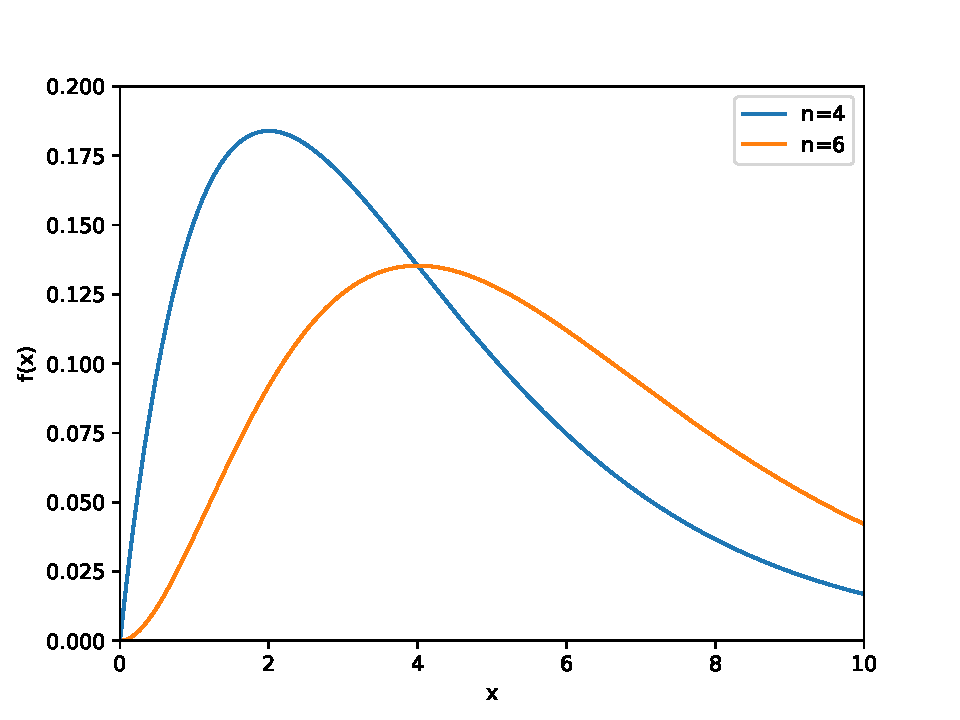
\includegraphics[scale=0.6]{./figure/chi.pdf}\end{center}
$\chi^2$分布性质:
\begin{enumerate}
\item 设$\chi_1^2\sim\chi^2\left(n_1\right)$,$\chi_2^2\sim\chi^2\left(n_2\right)$,且$\chi_1^2$和$\chi_2^2$相互独立,则有
\[\chi_1^2+\chi_2^2\sim\chi^2\left(n_1+n_2\right)\]
\item 设$\chi^2\sim\chi^2\left(n\right)$,则有
\[E\left(\chi^2\right)=n,\ D\left(\chi^2\right)=2n\]
\item 设总体$X\sim N\left(\mu,\sigma^2\right)$,$X_1,X_2,\cdots,X_n$是来自总体$X$的样本,则
\[\frac{\sum\limits_{i=1}^{n}\left(X_i-\mu\right)^2}{\sigma^2}\sim\chi^2\left(n\right)\]
\item 设$\chi^2\sim\chi^2\left(n\right)$,对于给定的正数$\alpha\in\left(0,1\right)$,则满足
\[P\left\{\chi^2>\chi_{\alpha}^2\left(n\right)\right\}=\alpha\]
的点$x=\chi_{\alpha}^2\left(n\right)$称为$\chi^2$的上$\alpha$分位点
\begin{center}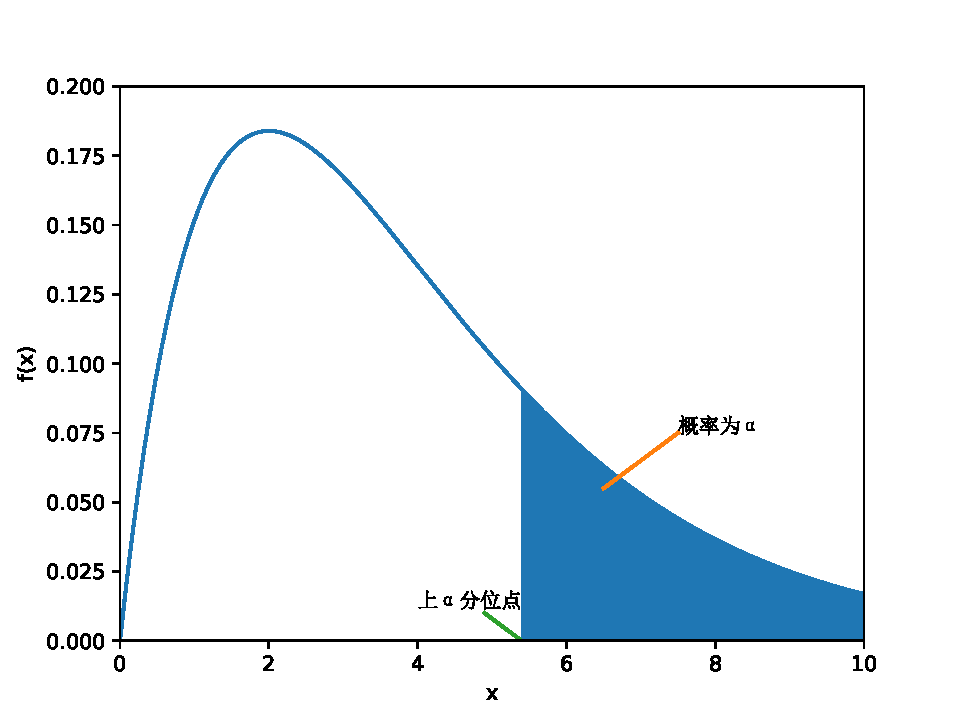
\includegraphics[scale=0.6]{./figure/chi_alpha.pdf}\end{center}
\end{enumerate}
\item \textbf{$t$分布}:设$X\sim N\left(0,1\right),\ Y\sim\chi^2\left(n\right)$,且$X,\ Y$相互独立,则称随机变量
\[t=\frac{X}{\sqrt{\frac{Y}{n}}}\]
服从自由度为$n$的$t$分布,记为$t\sim t\left(n\right)$,概率密度函数为
\[f\left(x\right)=\dfrac{\Gamma\left(\dfrac{n+1}{2}\right)}{\sqrt{n\pi}\cdot\Gamma\left(\dfrac{n}{2}\right)}\left(1+\dfrac{x^2}{n}\right)^{-\frac{n+1}{2}}\]
函数图像为:
\begin{center}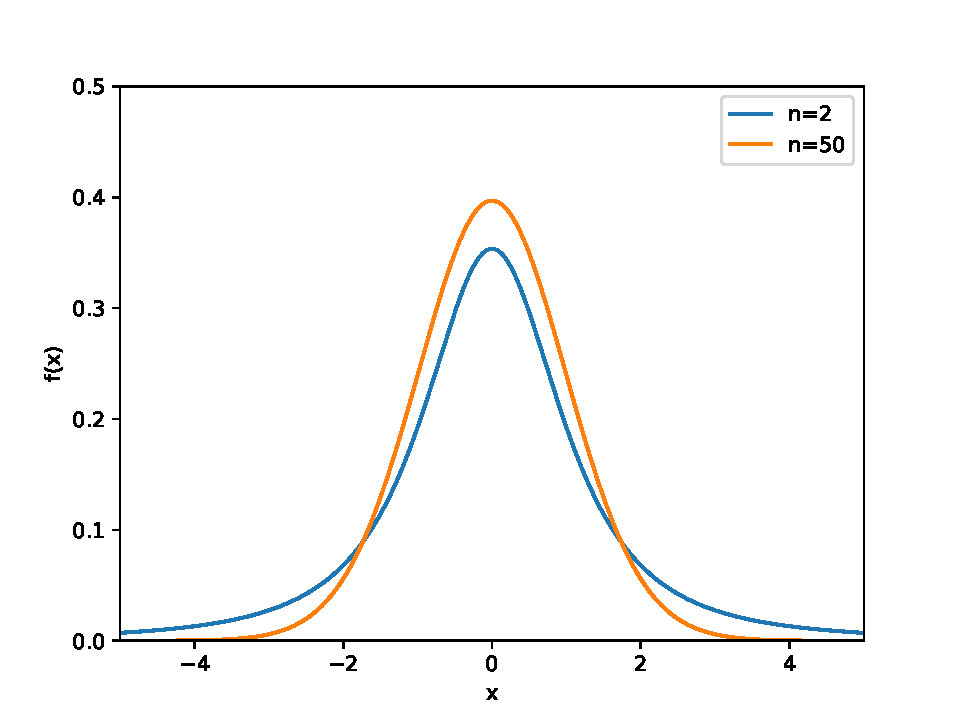
\includegraphics[scale=0.6]{./figure/t.pdf}\end{center}
$t$分布性质:
\begin{enumerate}
\item 对于$t$分布的密度函数$f\left(x\right)$我们有
\[\lim\limits_{n\to\infty}f\left(x\right)=\frac{1}{\sqrt{2\pi}}e^{-\frac{x^2}{2}}\]
即当$n$足够大时$t$分布近似于标准正态分布$N\left(0,1\right)$
\item 设$t\sim t\left(n\right)$,对于给定的正数$\alpha\in\left(0,1\right)$,则满足
\[P\left\{t>t_{\alpha}\left(n\right)\right\}=\alpha\]
的点$x=t_{\alpha}\left(n\right)$称为$t$的上$\alpha$分位点
\begin{center}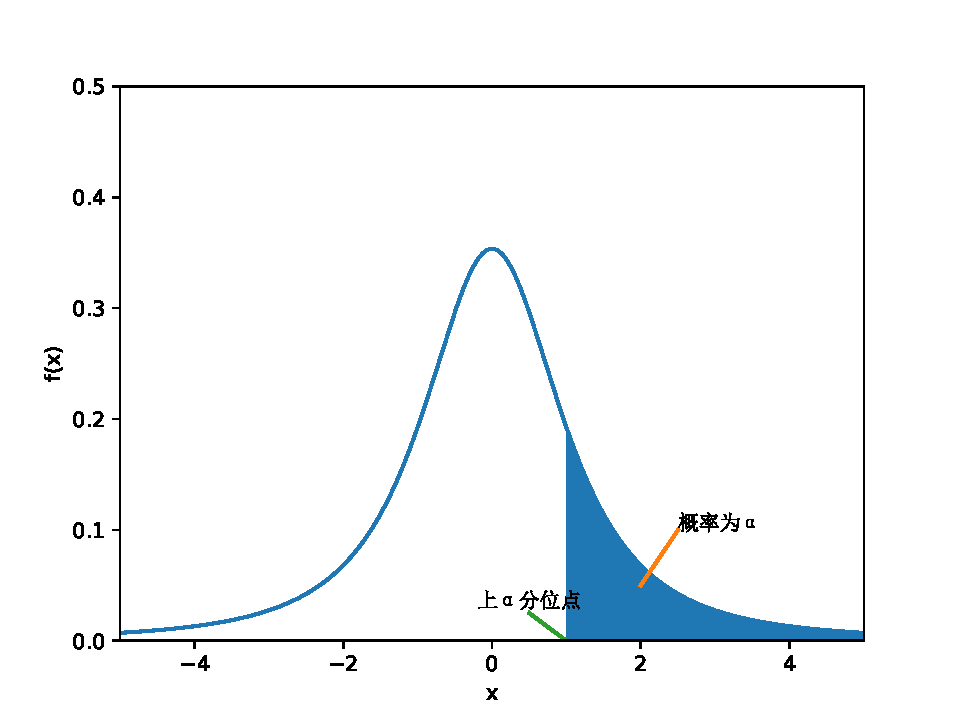
\includegraphics[scale=0.6]{./figure/t_alpha.pdf}\end{center}
\end{enumerate}
\item \textbf{$F$分布}:设$U\sim\chi^2\left(n_1\right),\ V\sim\chi^2\left(n_2\right)$,且$U,\ V$相互独立,则称随机变量
\[F=\frac{\ \frac{U}{n_1}\ }{\ \frac{V}{n_2}\ }\]
服从自由度为$\left(n_1,n_2\right)$的$F$分布,记为$F\sim F\left(n_1,n_2\right)$,概率密度函数为
\[f\left(x\right)=\left\{\begin{matrix}\dfrac{\Gamma\left(\dfrac{n_1+n_2}{2}\right)\cdot\left(\dfrac{n_1}{n_2}\right)^{\frac{n_1}{2}}\cdot x^{\frac{n_1}{2}-1}}{\Gamma\left(\dfrac{n_1}{2}\right)\cdot\Gamma\left(\dfrac{n_2}{2}\right)\cdot\left(1+\dfrac{n_1}{n_2}x\right)^{\frac{n_1+n_2}{2}}}\ ,&x>0\\0\ ,&else\end{matrix}\right.\]
函数图像为:
\begin{center}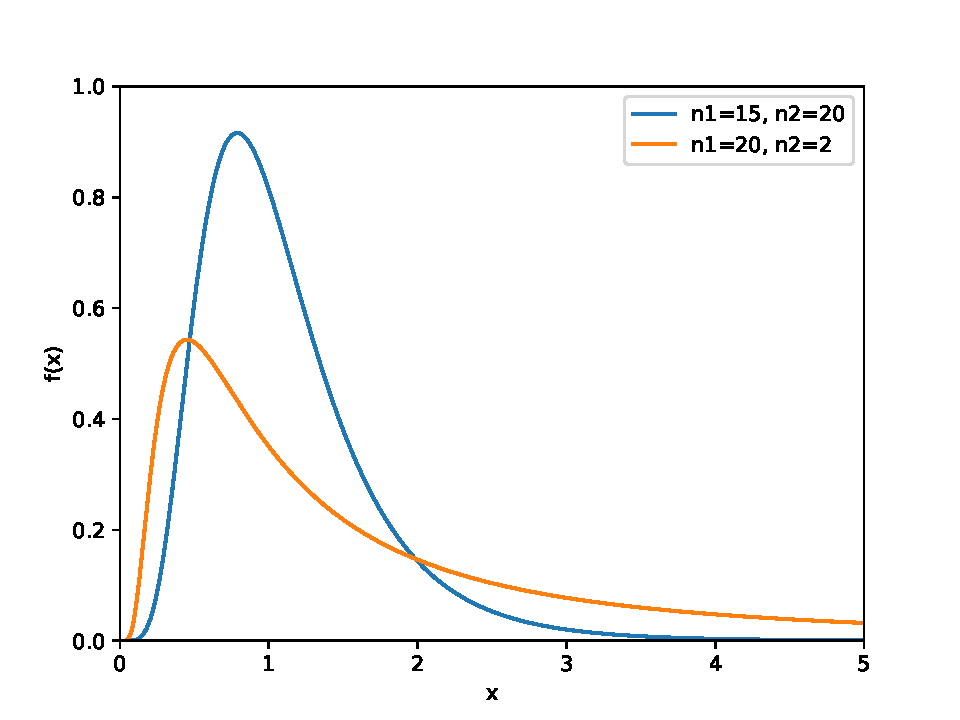
\includegraphics[scale=0.6]{./figure/F.pdf}\end{center}
$F$分布性质:
\begin{enumerate}
\item 若$F\sim F\left(n_1,n_2\right)$,则有
\[\frac{1}{F}\sim F\left(n_2,n_1\right)\]
\item 若$X\sim t\left(n\right)$,则$X^2\sim F\left(1,n\right)$
\item 设$F\sim F\left(n_1,n_2\right)$,对于给定的正数$\alpha\in\left(0,1\right)$,则满足
\[P\left\{F>F_{\alpha}\left(n_1,n_2\right)\right\}=\alpha\]
的点$x=F_{\alpha}\left(n_1,n_2\right)$称为$F$的上$\alpha$分位点
\begin{center}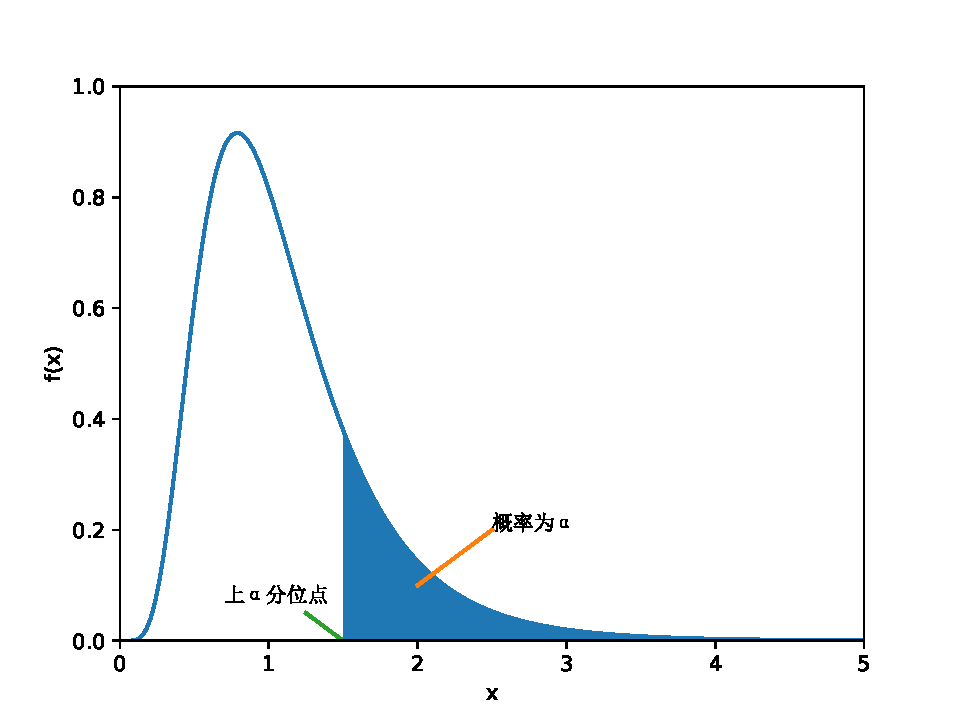
\includegraphics[scale=0.6]{./figure/F_alpha.pdf}\end{center}
\end{enumerate}
\end{enumerate}

\subsection{抽样分布样本均值和方差的分布}
\begin{enumerate}
\item 设总体$X$具有均值$\mu$和方差$\sigma^2$,$X_1,X_2,\cdots,X_n$是来自$X$的一个样本,$\overline{X}$和$S^2$分别是样本均值和样本方差,则我们有
\[E\left(\overline{X}\right)=\mu,\ D\left(\overline{X}\right)=\frac{\sigma^2}{n},\ E\left(S^2\right)=\sigma^2\]
\item \textbf{单个正态总体样本均值分布}:设$X_1,X_2,\cdots,X_n$是来自正态总体$N\left(\mu,\sigma^2\right)$的一个样本,$\overline{X}$是样本均值,则有
\[\overline{X}\sim N\left(\mu,\frac{\sigma^2}{n}\right)\]
\item \textbf{两个正态总体样本均值分布}:设$X_1,X_2,\cdots,X_m$与$Y_1,Y_2,\cdots,Y_n$分别是来自正态总体$N\left(\mu_1,\sigma_1^2\right)$ 和$N\left(\mu_2,\sigma_2^2\right)$的样本,且这两个正态总体$N\left(\mu_1,\sigma_1^2\right)$ 和$N\left(\mu_2,\sigma_2^2\right)$相互独立,$\overline{X},\overline{Y}$分别是其样本均值,则有
\[\overline{X}\pm\overline{Y}\sim N\left(\mu_1\pm\mu_2,\frac{\sigma_1^2}{m}+\frac{\sigma_2^2}{n}\right)\]
\item \textbf{非正态总体样本均值近似分布}:设$X_1,X_2,\cdots,X_n$是来自任意总体$X$的一个样本,总体的期望为$E\left(X\right)=\mu$,方差为$D\left(X\right)=\sigma^2$,则当$n$较大时,有
\[\overline{X}\sim N\left(\mu,\frac{\sigma^2}{n}\right)\]
\item 设$X_1,X_2,\cdots,X_n$是来自正态总体$N\left(\mu,\sigma^2\right)$的一个样本,$\overline{X}$和$S^2$分别是样本均值和样本方差,则$\overline{X}$和$S^2$相互独立,且有
\[\frac{\sum\limits_{i=1}^{n}\left(X_i-\overline{X}\right)^2}{\sigma^2}=\frac{\left(n-1\right)S^2}{\sigma^2}\sim\chi^2\left(n-1\right)\]
\item 设$X_1,X_2,\cdots,X_n$是来自正态总体$N\left(\mu,\sigma^2\right)$的一个样本,$\overline{X}$和$S^2$分别是样本均值和样本方差,则有
\[\frac{\overline{X}-\mu}{\frac{S}{\sqrt{n}}}\sim t\left(n-1\right)\]
\item 设$X_1,X_2,\cdots,X_{n_1}$与$Y_1,Y_2,\cdots,Y_{n_2}$分别是来自正态总体$N\left(\mu_1,\sigma_1^2\right)$和$N\left(\mu_2,\sigma_2^2\right)$的样本,且这两个正态总体$N\left(\mu_1,\sigma_1^2\right)$ 和$N\left(\mu_2,\sigma_2^2\right)$相互独立,$\overline{X},\overline{Y}$ 和$S_1^2,S_2^2$分别是样本均值和样本方差,则有
\[\frac{\ \frac{S_1^2}{S_2^2}\ }{\ \frac{\sigma_1^2}{\sigma_2^2}\ }\sim F\left(n_1-1,n_2-1\right)\]
而当$\sigma_1^2=\sigma_2^2=\sigma^2$时,还有
\[\frac{\left(\overline{X}-\overline{Y}\right)-\left(\mu_1-\mu_2\right)}{\sqrt{\frac{\left(n_1-1\right)S_1^2+\left(n_2-1\right)S_2^2}{n_1+n_2-2}}\cdot\sqrt{\frac{1}{n_1}+\frac{1}{n_2}}}\sim t\left(n_1+n_2-2\right)\]
\end{enumerate}


\section{参数估计}
\subsection{矩估计}
\begin{enumerate}
\item \textbf{样本原点矩与中心矩}:对于总体$X$,设$X_1,X_2,\cdots,X_n$为其样本,则样本原点矩与中心矩定义为:
\begin{enumerate}
\item 样本$k$阶原点矩:
\[A_k=\frac{1}{n}\sum\limits_{i=1}^{n}X_i^k\]
\item 样本$k$阶中心矩:
\[B_k=\frac{1}{n}\sum\limits_{i=1}^{n}\left(X_i-\overline{X}\right)^k\]
\end{enumerate}
\item \textbf{矩估计定义}:表示总体原点矩或中心矩与未知参数关系的函数方程(组)
\[\left\{\begin{aligned}
\theta_1&=\theta_1\left(\mu_1,\mu_2,\cdots,\mu_k\right)\\
\theta_2&=\theta_2\left(\mu_1,\mu_2,\cdots,\mu_k\right)\\
&\vdots\\
\theta_k&=\theta_k\left(\mu_1,\mu_2,\cdots,\mu_k\right)
\end{aligned}\right.\]
称为矩估计方程(组),用对应的样本矩替代方程组中的总体矩后得到的
\[\hat{\theta}_i=\theta_i\left(A_1,A_2,\cdots,A_k\right)\]
分别称为$\theta_i$的矩估计量,矩估计量的观察值称为矩估计值
\item \textbf{矩估计性质}:
\begin{enumerate}
\item 若$\hat{\theta}$为参数$\theta$的矩估计量,$g\left(x\right)$为$x$的连续函数,则$g\left(\hat{\theta}\right)$是$g\left(\theta\right)$的矩估计量
\item 若$\hat{\theta}_1,\ \hat{\theta}_2$为参数$\theta_1,\ \theta_2$的矩估计量,$g\left(x,y\right)$为$\left(x,y\right)$的连续函数,则$g\left(\hat{\theta}_1,\hat{\theta}_2\right)$是$g\left(\theta_1,\theta_2\right)$的矩估计量
\end{enumerate}
\end{enumerate}

\subsection{极大似然估计}
\begin{enumerate}
\item \textbf{单参数似然函数}:对于总体$X$,设$f\left(x;\theta\right)$为总体$X$的概率密度函数,其中$\theta$是未知参数,$X_1,X_2,\cdots,X_n$为总体$X$的一个样本,则自变量为$\theta$,定义域为$\varTheta$的非负函数
\[L\left(x_1,x_2,\cdots,x_n;\theta\right)=\prod\limits_{i=1}^{n}f\left(x_i;\theta\right),\ \theta\in\varTheta\]
称为容量为$n$的样本似然函数,或称为样本值$x_1,x_2,\cdots,x_n$的似然函数
\item \textbf{单参数极大似然估计}:对于总体$X$,设$X_1,X_2,\cdots,X_n$为其样本,若存在$\hat{\theta}=\hat{\theta}\left(x_1,x_2,\cdots,x_n\right)$,使
\[L\left(\hat{\theta}\right)=\max\limits_{\theta\in\varTheta}L\left(\theta\right)\]
则称似然函数的最大值点$\hat{\theta}\left(x_1,x_2,\cdots,x_n\right)$为参数$\theta$的极大似然估计值,而称$\hat{\theta}\left(X_1,X_2,\cdots,X_n\right)$为参数$\theta$的极大似然估计量
\item \textbf{多参数似然函数}:对于总体$X$,设$f\left(x;\theta_1,\theta_2,\cdots,\theta_m\right)$为总体$X$的概率密度函数,其中$\theta_i$是未知参数,$X_1,X_2,\cdots,X_n$为总体$X$的一个样本,则自变量为$\theta_1,\theta_2,\cdots,\theta_m$,定义域为$\varTheta^m$的非负函数
\[L\left(x_1,x_2,\cdots,x_n;\theta_1,\theta_2,\cdots,\theta_m\right)=\prod\limits_{i=1}^{n}f\left(x_i;\theta_1,\theta_2,\cdots,\theta_m\right),\ \left(\theta_1,\theta_2,\cdots,\theta_m\right)\in\varTheta^m\]
称为容量为$n$的样本似然函数,或称为样本值$x_1,x_2,\cdots,x_n$的似然函数
\item \textbf{多参数极大似然估计}:对于总体$X$,设$X_1,X_2,\cdots,X_n$为其样本,若存在一组$\hat{\theta}_i=\hat{\theta}_i\left(x_1,x_2,\cdots,x_m\right)$,使
\[L\left(\hat{\theta}_1,\hat{\theta}_2,\cdots,\hat{\theta}_m\right)=\max\limits_{\left(\theta_1,\theta_2,\cdots,\theta_m\right)\in\varTheta^m}L\left(\theta_1,\theta_2,\cdots,\theta_m\right)\]
则称似然函数的最大值点$\hat{\theta}_i\left(x_1,x_2,\cdots,x_n\right)$为参数$\theta_i$的极大似然估计值,而称$\hat{\theta}_i\left(X_1,X_2,\cdots,X_n\right)$为参数$\theta_i$的极大似然估计量
\item \textbf{极大似然估计性质}:
\begin{enumerate}
\item 若$\hat{\theta}$为参数$\theta$的极大似然估计量,$g\left(x\right)$为$x$的连续函数,则$g\left(\hat{\theta}\right)$是$g\left(\theta\right)$的极大似然估计量
\item 若$\hat{\theta}_1,\ \hat{\theta}_2$为参数$\theta_1,\ \theta_2$的极大似然估计量,$g\left(x,y\right)$为$\left(x,y\right)$的连续函数,则$g\left(\hat{\theta}_1,\hat{\theta}_2\right)$是$g\left(\theta_1,\theta_2\right)$的极大似然估计量
\item 若任意总体$X$的数学期望和方差均存在,则其数学期望的矩估计量和极大似然估计量相同,均为$\frac{1}{n}\sum\limits_{i=1}^{n}X_i$;其方差的矩估计量和极大似然估计量也相同,均为$\frac{1}{n}\sum\limits_{i=1}^{n}\left(X_i-\overline{X}\right)^2$
\end{enumerate}
\end{enumerate}

\subsection{估计量无偏性、有效性、一致性}
\begin{enumerate}
\item \textbf{无偏性}:设$\hat{\theta}$是未知参数$\theta$的估计量,若$E\left(\hat{\theta}\right)=\theta$,则称$\hat{\theta}$是$\theta$的无偏估计量
\item \textbf{有效性}:设$\hat{\theta}_1\left(X_1,X_2,\cdots,X_n\right)$与$\hat{\theta}_2\left(X_1,X_2,\cdots,X_n\right)$均为$\theta$的无偏估计量,若有
\[D\left(\hat{\theta}_1\right)<D\left(\hat{\theta}_2\right)\]
则称$\hat{\theta}_1$比$\hat{\theta}_2$更有效
\item \textbf{一致性(相合性)}:设$\hat{\theta}_n\left(X_1,X_2,\cdots,X_n\right)$为参数$\theta$的估计量,若对任意$\theta\in\varTheta$,当样本容量$n\to\infty$时,$\hat{\theta}_n\left(X_1,X_2,\cdots,X_n\right)$依概率收敛于$\theta$,即对任意$\varepsilon>0$,有
\[\lim\limits_{n\to\infty}P\left(\left|\hat{\theta}_n-\theta\right|\geq\varepsilon\right)=0\]
则称$\hat{\theta}_n$为$\theta$一致估计量,也叫相合估计量
\item \textbf{性质}:
\begin{enumerate}
\item 设$\hat{\theta}_n$为$\theta$无偏估计量,且$\lim\limits_{n\to\infty}D\left(\hat{\theta}_n\right)=0$,则$\hat{\theta}_n$为$\theta$一致估计量
\item 设$\hat{\theta}_n$为$\theta$的一致估计量,若函数$g\left(x\right)$连续,则$g\left(\hat{\theta}_n\right)$为$g\left(\theta\right)$的一致估计量
\item 任意样本原点矩是总体原点矩的一致估计量。进一步地,若待估参数$\theta=g\left(\mu_1,\mu_2,\cdots,\mu_k\right)$,而函数$g$连续,则矩估计量$\hat{\theta}=g\left(A_1,A_2,\cdots,A_k\right)$为$\theta$的一致估计量
\end{enumerate}
\end{enumerate}

\subsection{正态总体参数的区间估计}
\begin{enumerate}
\item 一个正态总体
\begin{enumerate}
\item \textbf{待估参数为$\mu$,且$\sigma^2$已知时}:\\
用作估计的随机变量及其分布为:
\[Z=\frac{\overline{X}-\mu}{\frac{\sigma}{\sqrt{n}}}\sim N\left(0,1\right)\]
置信度为$1-\alpha$的置信区间为:
\[\left(\overline{X}\pm\frac{\sigma}{\sqrt{n}}z_{\frac{\alpha}{2}}\right)\]
单侧置信限为:
\[\underline{\mu}=\overline{X}-\frac{\sigma}{\sqrt{n}}z_{\alpha}\]
\[\overline{\mu}=\overline{X}+\frac{\sigma}{\sqrt{n}}z_{\alpha}\]
\item \textbf{待估参数为$\mu$,且$\sigma^2$未知时}:\\
用作估计的随机变量及其分布为:
\[t=\frac{\overline{X}-\mu}{\frac{S}{\sqrt{n}}}\sim t\left(n-1\right)\]
置信度为$1-\alpha$的置信区间为:
\[\left(\overline{X}\pm\frac{S}{\sqrt{n}}t_{\frac{\alpha}{2}}\left(n-1\right)\right)\]
单侧置信限为:
\[\underline{\mu}=\overline{X}-\frac{S}{\sqrt{n}}t_{\alpha}\left(n-1\right)\]
\[\overline{\mu}=\overline{X}+\frac{S}{\sqrt{n}}t_{\alpha}\left(n-1\right)\]
\item \textbf{待估参数为$\sigma^2$,且$\mu$未知时}:\\
用作估计的随机变量及其分布为:
\[\chi^2=\frac{\left(n-1\right)S^2}{\sigma^2}\sim\chi^2\left(n-1\right)\]
置信度为$1-\alpha$的置信区间为:
\[\left(\frac{\left(n-1\right)S^2}{\chi_{\frac{\alpha}{2}}^2\left(n-1\right)},\frac{\left(n-1\right)S^2}{\chi_{1-\frac{\alpha}{2}}^2\left(n-1\right)}\right)\]
单侧置信限为:
\[\underline{\sigma^2}=\frac{\left(n-1\right)S^2}{\chi_{\alpha}^2\left(n-1\right)}\]
\[\overline{\sigma^2}=\frac{\left(n-1\right)S^2}{\chi_{1-\alpha}^2\left(n-1\right)}\]
\end{enumerate}
\item 两个正态总体
\begin{enumerate}
\item \textbf{待估参数为$\mu_1-\mu_2$,且$\sigma_1^2,\sigma_2^2$已知时}:\\
用作估计的随机变量及其分布为:
\[Z=\frac{\left(\overline{X}-\overline{Y}\right)-\left(\mu_1-\mu_2\right)}{\sqrt{\frac{\sigma_1^2}{n_1}+\frac{\sigma_2^2}{n_2}}}\sim N\left(0,1\right)\]
置信度为$1-\alpha$的置信区间为:
\[\left(\left(\overline{X}-\overline{Y}\right)\pm\sqrt{\frac{\sigma_1^2}{n_1}+\frac{\sigma_2^2}{n_2}}\cdot z_{\frac{\alpha}{2}}\right)\]
单侧置信限为:
\[\underline{\mu_1-\mu_2}=\left(\overline{X}-\overline{Y}\right)-\sqrt{\frac{\sigma_1^2}{n_1}+\frac{\sigma_2^2}{n_2}}\cdot z_{\alpha}\]
\[\overline{\mu_1-\mu_2}=\left(\overline{X}-\overline{Y}\right)+\sqrt{\frac{\sigma_1^2}{n_1}+\frac{\sigma_2^2}{n_2}}\cdot z_{\alpha}\]
\item \textbf{待估参数为$\mu_1-\mu_2$,且$\sigma_1^2=\sigma_2^2=\sigma^2$未知时}:\\
用作估计的随机变量及其分布为:
\[\frac{\left(\overline{X}-\overline{Y}\right)-\left(\mu_1-\mu_2\right)}{\sqrt{\frac{\left(n_1-1\right)S_1^2+\left(n_2-1\right)S_2^2}{n_1+n_2-2}}\cdot\sqrt{\frac{1}{n_1}+\frac{1}{n_2}}}\sim t\left(n_1+n_2-2\right)\]
置信度为$1-\alpha$的置信区间为:
\[\left(\left(\overline{X}-\overline{Y}\right)\pm\sqrt{\frac{\left(n_1-1\right)S_1^2+\left(n_2-1\right)S_2^2}{n_1+n_2-2}}\cdot\sqrt{\frac{1}{n_1}+\frac{1}{n_2}}\cdot t_{\frac{\alpha}{2}}\left(n_1+n_2-2\right)\right)\]
单侧置信限为:
\[\underline{\mu_1-\mu_2}=\left(\overline{X}-\overline{Y}\right)-\sqrt{\frac{\left(n_1-1\right)S_1^2+\left(n_2-1\right)S_2^2}{n_1+n_2-2}}\cdot\sqrt{\frac{1}{n_1}+\frac{1}{n_2}}\cdot t_{\alpha}\left(n_1+n_2-2\right)\]
\[\overline{\mu_1-\mu_2}=\left(\overline{X}-\overline{Y}\right)+\sqrt{\frac{\left(n_1-1\right)S_1^2+\left(n_2-1\right)S_2^2}{n_1+n_2-2}}\cdot\sqrt{\frac{1}{n_1}+\frac{1}{n_2}}\cdot t_{\alpha}\left(n_1+n_2-2\right)\]
\item \textbf{待估参数为$\dfrac{\sigma_1^2}{\sigma_2^2}$,且$\mu_1,\mu_2$未知时}:\\
用作估计的随机变量及其分布为:
\[\frac{\ \frac{S_1^2}{S_2^2}\ }{\ \frac{\sigma_1^2}{\sigma_2^2}\ }\sim F\left(n_1-1,n_2-1\right)\]
置信度为$1-\alpha$的置信区间为:
\[\left(\frac{S_1^2}{S_2^2}\cdot\frac{1}{F_{\frac{\alpha}{2}}\left(n_1-1,n_2-1\right)},\frac{S_1^2}{S_2^2}\cdot\frac{1}{F_{1-\frac{\alpha}{2}}\left(n_1-1,n_2-1\right)}\right)\]
单侧置信限为:
\[\underline{\left(\frac{\sigma_1^2}{\sigma_2^2}\right)}=\frac{S_1^2}{S_2^2}\cdot\frac{1}{F_{\alpha}\left(n_1-1,n_2-1\right)}\]
\[\overline{\left(\frac{\sigma_1^2}{\sigma_2^2}\right)}=\frac{S_1^2}{S_2^2}\cdot\frac{1}{F_{1-\alpha}\left(n_1-1,n_2-1\right)}\]
\end{enumerate}
\item 一些性质
\begin{enumerate}
\item 若$\left[\underline{\theta},\overline{\theta}\right]$为$\theta$的置信度为$1-\alpha$的置信区间,$g\left(x\right)$为单调函数,则$\left[g\left(\underline{\theta}\right),g\left(\overline{\theta}\right)\right]$(或$\left[g\left(\overline{\theta}\right),g\left(\underline{\theta}\right)\right]$)为$g\left(\theta\right)$的置信度为$1-\alpha$的置信区间
\end{enumerate}
\end{enumerate}











\chapter{解题笔记}

\section{多维随机变量及其分布}
\begin{enumerate}
\item 离散型随机变量和连续型随机变量混合\\
例:设随机变量$X$与$Y$独立,其中$X$的概率分布为
\[X\sim\begin{bmatrix}1&2\\0.3&0.7\end{bmatrix}\]
而$Y$的概率密度为$f\left(Y\right)$,求随机变量$U=X+Y$的概率密度$g\left(u\right)$\\
解:设$F\left(y\right)$是$Y$的分布函数,则由全概公式以及$X$和$Y$相互独立知$U=X+Y$的分布函数为
\[\begin{aligned}
G\left(u\right)&=P\left(X+Y\leq u\right)\\
&=0.3P\left(X+Y\leq u|X=1\right)+0.7P\left(X+Y\leq u|X=2\right)\\
&=0.3P\left(Y\leq u-1|X=1\right)+0.7P\left(Y\leq u-2|X=2\right)\\
&=0.3P\left(Y\leq u-1\right)+0.7P\left(Y\leq u-2\right)\\
&=0.3F\left(u-1\right)+0.7F\left(u-2\right)
\end{aligned}\]
因此$U=X+Y$的概率密度为
\[g\left(u\right)=G^{\prime}\left(u\right)=0.3f\left(u-1\right)+0.7f\left(u-2\right)\]
\end{enumerate}


\section{随机变量的数字特征}
\begin{enumerate}
\item 利用随机变量分解法和数字特征运算规律求解数字特征\\
例:将$n$个球($1\sim n$号)随机放进$n$个盒子($1\sim n$号)中去,一个盒子装一个球,将一个球装入与球同号的盒子中称为一个配对,记$X$为总的配对数,求$E\left(X\right)$\\
解:记随机变量$X_i$为$i$号球的配对数,显然每个球的配对数只有$1$和$0$两种可能,而尽管随机变量$X_i$互相并不独立,但我们有$P\left(X_i=1\right)=\frac{1}{n}$,而又因为$X=\sum\limits_{i=1}^{n}X_i$,故我们有
\[E\left(X\right)=\sum\limits_{i=1}^{n}E\left(X_i\right)=n\cdot\frac{1}{n}=1\]
\end{enumerate}





\end{document}









